\chapter{Blockchain e Bitcoin}
\section{Blockchain}
La blockchain (letteralmente "catena di blocchi") è una struttura dati condivisa e "immutabile". È definita come
un registro digitale le cui voci sono raggruppate in "blocchi", concatenati in ordine cronologico, e la cui integrità è
garantita dall'uso della crittografia. Sebbene la sua dimensione sia destinata a crescere nel tempo, è immutabile
in quanto, di norma, il suo contenuto una volta scritto non è più né modificabile né eliminabile, a meno di non
invalidare l'intera struttura.

\singlespacing

Tali tecnologie sono incluse nella più ampia famiglia delle “Distributed Ledger”, ossia sistemi che si basano su un
registro distribuito, che può essere letto e modificato da più nodi di una rete. Non è richiesto che i nodi coinvolti
conoscano l'identità reciproca o si fidino l'uno dell'altro. Difatti, per garantire la coerenza tra le varie copie,
l'aggiunta di un nuovo blocco è globalmente regolata da un protocollo condiviso. Una volta autorizzata l'aggiunta
del nuovo blocco, ogni nodo aggiorna la propria copia privata: la natura stessa della struttura dati garantisce
l'assenza di una sua manipolazione futura. Le caratteristiche che accomunano i sistemi sviluppati con le tecnologie
Blockchain e Distributed Ledger sono digitalizzazione dei dati, decentralizzazione, disintermediazione, tracciabilità
dei trasferimenti, trasparenza/verificabilità, immutabilità del registro e programmabilità dei trasferimenti.[
Grazie a tali caratteristiche, la blockchain è considerata pertanto un'alternativa in termini di sicurezza, affidabilità,
trasparenza e costi alle banche dati e ai registri gestiti in maniera centralizzata da autorità riconosciute e
regolamentate (pubbliche amministrazioni, banche, assicurazioni, intermediari di pagamento, ecc.)

\singlespacing

\paragraph{Descrizione:} Una blockchain è un registro digitale aperto e distribuito, in grado di memorizzare record di dati (solitamente, denominati "transazioni") in modo sicuro, verificabile e permanente. Una volta scritti, i dati in un blocco non possono essere retroattivamente alterati senza che vengano modificati tutti i blocchi successivi ad esso e ciò, per
la natura del protocollo e dello schema di validazione, necessiterebbe del consenso della maggioranza della
rete. La blockchain è quindi rappresentabile come una lista, in continua crescita, di "blocchi" collegati tra loro e
resi sicuri mediante l'uso della crittografia. Ad un blocco possono essere associate una o più transazioni e ogni
blocco, inoltre, contiene un puntatore hash al blocco precedente e una marca temporale.
La natura distribuita e il modello cooperativo rendono robusto e sicuro il processo di validazione, ma presentano
tempi non trascurabili, dovuti in gran parte al processo di validazione dei blocchi e alla sincronizzazione delle
rete. L'autenticazione avviene tramite collaborazione di massa ed è alimentata da interessi collettivi. L'utilizzo di
questa tecnologia consente anche di superare il problema dell'infinita riproducibilità di un bene digitale e
della doppia spesa, senza l'utilizzo di un server centrale o di un'autorità.
Talvolta risulta possibile che alcuni nodi della rete producano simultaneamente più blocchi "concorrenti" (ossia
collegati a uno stesso blocco già esistente, ma diversi tra loro nel contenuto): ciò dà origine a una biforcazione
(fork) nella catena. Il protocollo di aggiornamento specifica quale regola i nodi debbano adottare per selezionare
il blocco da accettare, tra quelli concorrenti. I blocchi non selezionati per l'inclusione nella catena sono chiamati
"blocchi orfani"

\section{Bitcoin}
Il bitcoin si comporta più come “oro” che come “moneta” perché il valore cambia nel tempo. Più che proprietà o
possesso di bitcoin/monete si parla di diritto di spesa, che si ottiene conoscendo una determinata chiave di
cifratura.

\singlespacing

Come faccio a ricevere bitcoin? Utilizzando un exchange (piattaforma per lo scambio di criptovalute) si ha la
possibilità di inviare/ricevere queste chiavi di cifratura segrete che determinano il diritto di possesso di un certo
numero di monete/criptovalute virtuali.

\singlespacing

Esempio transazione fatto a lezione:

\begin{itemize}
    \item A paga in euro
    
    \item A comunica la propria chiave pubblica
    
    \item B riceve gli euro da A e cede i suoi bitcoin
    
    \item La cessione avviene sbloccando i bitcoin dalla chiave privata di B per poi assegnarli alla chiave pubblica di A
    
    \item Il nuovo proprietario è A perché è l’unico ad avere una determinata chiave privata associata ad una determinata chiave pubblica
\end{itemize}
Le chiavi pubbliche e private sono associate 1 a 1, conoscendo la chiave pubblica non è possibile conoscere la
chiave privata e viceversa.
Quindi nell’esempio io genero una coppia chiave pubblica-privata, divulgo la pubblica e ci ottengo i bitcoin sopra
che poi con la chiava privata potrò spendere o cedere a qualcun altro.

Il Bitcoin (codice: BTC o XBT) è una criptovaluta e un sistema di pagamento mondiale creato
nel 2009 da un anonimo inventore (o gruppo di inventori), noto con lo pseudonimo di Satoshi Nakamoto (|| in
realtà si dice che ci fosse dietro un intero team), che sviluppò un'idea da lui stesso presentata su Internet a
fine 2008. Per convenzione se il termine Bitcoin è utilizzato con l'iniziale maiuscola si riferisce alla tecnologia e
alla rete, mentre se minuscola (bitcoin) si riferisce alla valuta in sé.

\singlespacing

Dagli esperti di finanza il Bitcoin non viene classificato come una moneta, ma come una riserva di valore
attualmente molto volatile. A differenza della maggior parte delle valute tradizionali, il Bitcoin non fa uso di un ente
centrale né di meccanismi finanziari sofisticati, il valore è determinato unicamente dalla leva domanda e offerta:
esso utilizza un database distribuito tra i nodi della rete che tengono traccia delle transazioni, ma sfrutta
la crittografia per gestire gli aspetti funzionali, come la generazione di nuova moneta e l'attribuzione
della proprietà dei bitcoin.

\singlespacing

La rete Bitcoin consente il possesso e il trasferimento pseudo-anonimo delle monete; i dati necessari a utilizzare
i propri bitcoin possono essere salvati su uno o più personal computer o dispositivi elettronici quali smartphone,
sotto forma di "portafoglio" digitale, o mantenuti presso terze parti che svolgono funzioni simili a una banca. Il
wallet bitcoin ha un indirizzo identificato da un codice alfanumerico che possiede tra i 25 e i 36 caratteri tra
numeri e lettere; è l'unico dato da comunicare per ricevere un pagamento che godrà di un certo grado di
anonimato, ma sarà allo stesso tempo pubblicamente e immutabilmente visibile sulla blockchain per sempre.
Occorre fare molta attenzione nella trasmissione del codice alfanumerico in quanto eventuali errori non consentono
di annullare l'operazione e causano la perdita del denaro. È possibile ricevere pagamenti più semplicemente
attraverso la scansione di codici QR. In ogni caso, i bitcoin possono essere trasferiti attraverso Internet verso
chiunque disponga di un "indirizzo bitcoin". La struttura peer-to-peer della rete Bitcoin e la mancanza di un ente
centrale rende impossibile a qualunque autorità, governativa o meno, il blocco dei trasferimenti, il sequestro di
bitcoin senza il possesso delle relative chiavi o la svalutazione dovuta all'immissione di nuova moneta.
Il Bitcoin è una delle prime implementazioni di un concetto definito come criptovaluta, descritto per la prima volta
nel 1998 da Wei Dai su una mailing list.

\singlespacing

BitCoin è una scoperta informatica che definisce e implementa un sistema di pagamento sicuro e
decentralizzato e uno strumento per l'archiviazione, la verifica e la revisione delle informazioni, comprese le
rappresentazioni digitali dei valori.
Il protocollo bitcoin definisce una rete overlay su Internet che estrae bitcoin, ogni nodo gestisce un gruppo di
indirizzi che detiene monete, ogni indirizzo è un'immagine hash di una sottostante coppia privata-pubblica
di chiavi crittografiche e agisce come uno pseudonimo del titolare della moneta.
La visione dei nodi di questo stato comune è formata da una BlockChain, un libro mastro condiviso, appendibile,
affidabile, di tutte le transazioni delle monete. I limiti del consenso distribuito definiti nel Problema Bizantino e nel
Teorema CAP sono risolti usando la tecnica del proof-of-work.

\singlespacing

Il bitcoin, visto soprattutto il continuo incremento/decremento del proprio valore, viene difficilmente considerato
spendibile. Esiste una versione chiamata bitcoin cash che riesce a mantenere di più il valore nel tempo, perciò
viene consideratà “più spendibile”.
Con i bitcoin non c’è nessuna terza parte fidata per eseguire le operazioni peer-to-peer, per esempio le banche.
Per avere una garanzia che la transazione venga registrata in tempo breve bisogna pagare una commissione,
questa commissione verrà incassata da chi si occupa di questo tipo di operazioni, ovvero i miner.
\subsection{Bitcoin core}
Il software Bitcoin Core (evoluzione Bitcoin-Qt) può essere scaricato come qualsiasi altro programma sul nostro
computer. Ma prima di ciò, è necessario tenere conto di diversi aspetti. Primo, Bitcoin Core implementa tutti gli
aspetti della rete Bitcoin, quindi scaricarlo ti renderà un nodo completo della rete. Ciò include una copia esatta
e completa di tutte le operazioni che sono state effettuate con Bitcoin dal suo lancio nel 2009. E,
naturalmente, sarà costantemente aggiornato. Quindi la richiesta di spazio di archiviazione disponibile sul disco
rigido sarà di almeno 400 GB.

\singlespacing

Secondo Bitcoin Core implementa un wallet, attraverso il quale tutte le transazioni effettuate con la copia del
file blockchain. Quindi scaricarlo e sincronizzarlo su un computer richiederà alcuni giorni prima di poterlo utilizzare.
Pertanto, sebbene offra livelli elevati di sicurezza e privacy, è consigliato solo per utenti esperti.
Un'altra caratteristica importante di Bitcoin Core è che utilizza un programma interno (demone) chiamato bitcoind.
Un demone (demone in spagnolo) è un programma che viene eseguito in background per essere utilizzato tramite
le righe di comando e chiamate di procedura remota (RPC). Il nome "demone" è strettamente correlato ai
sistemi UNIX e derivati simili GNU / Linux. Bitcoin Core è anche in grado di creare un file testnet, una testnet in
cui gli sviluppatori controllano le modifiche che desiderano apportare. Pertanto, possono analizzare in dettaglio
come funzionano i cambiamenti o miglioramenti che desiderano per la rete prima di incorporarli in essa.
Inoltre, Bitcoin Core contiene anche un programma chiamato bitcoin-cli. Questa è un'interfaccia a riga di comando,
attraverso la quale gli utenti possono inviare comandi RPC a bitcoind ed eseguire qualsiasi operazione supportata
da Bitcoin.

\begin{figure}[H]
	\centering
    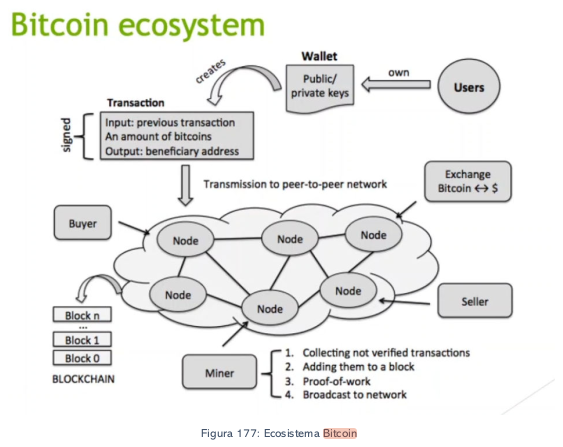
\includegraphics[width=14cm, keepaspectratio]{Bistarelli/img/bitcoin/bit1.png}
\end{figure}

Come rappresentato in Fig. 1, i principali attori della piattaforma sono gli utenti, che possiedono un portafoglio
associato ad una coppia di chiavi crittografiche private/pubbliche. Gli utenti usano queste chiavi per firmare
transazioni (irreversibili per progettazione), che sono poi trasmesse alla rete peer-to-peer Bitcoin. Alcuni dei pari
in questa rete sono i minatori, il cui compito è quello di aggiornare la blockchain, una struttura dati pubblica e
distribuita che implementa il database di ogni transazione mai eseguita.
Un proprietario di bitcoin trasferisce la moneta ad un altro proprietario (ad es, un acquirente a un venditore nella
Fig. 1 firmando digitalmente un hash di una transazione precedente (dimostrando che questo proprietario è in
possesso di bitcoin ricevuti in precedenza) e la chiave pubblica del prossimo proprietario. L'uso di input multipli
corrisponde all'uso di uso di più monete in una transazione in contanti. Una transazione può anche avere uscite
multiple, permettendo al proprietario di effettuare più pagamenti contemporaneamente. Un beneficiario può
verificare le firme per verificare la catena di proprietà. La somma delle entrate può superare la somma prevista dei
pagamenti, ma, come nelle transazioni in contanti, un uscita aggiuntiva è usata per restituire il resto al pagatore.
Le commissioni di transazione sono volontarie da parte di chi paga, e rappresentano solo un incentivo per i
minatori.

\singlespacing

Note immagine:

\begin{itemize}
    \item Exchange: trasformazione bitcoin e moneta
    
    \item Nodi per registrare transazioni
    
    \item Gli utenti che voglio partecipare all’ecosistema devo essere dotati di un wallet:
    
    \begin{itemize}
        \item Un wallet è un software che permette di gestire in maniera facile le copie di chiavi private-pubbliche, che servono per ricevere o dare diritti di spesa/transazioni
    \end{itemize}
    
    \item Le transazioni vengono salvate sui database distribuiti e vengono replicate su tutti i nodi della rete. Soprattutto per questo non serve una banca a verificare la validità delle transazioni, perché su ogni pc della rete sarà presente la prova della transazioni.
\end{itemize}

\begin{figure}[H]
	\centering
    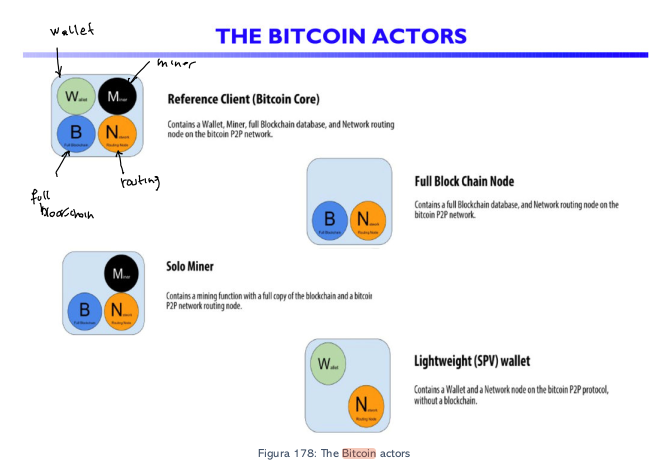
\includegraphics[width=14cm, keepaspectratio]{Bistarelli/img/bitcoin/bit2.png}
\end{figure}
Tipologia di nodi:
\begin{itemize}
    \item Wallet (verde): mantiene le chiavi pubbliche e private
    
    \begin{itemize}
        \item (Quando viene effettuata un’operazione viene messa in chiaro solo la chiave pubblica, ma non gli utenti mittenti e destinari coinvolti)
    \end{itemize}
    
    \item Routing (arancione): quando riceve una transazione può fare il broadcast in modo da comunicarlo a tutti
    
    \item Full blockchain (blu): tiene il database di tutte le transazioni fatte e/o può creare transazioni
    
    \item Miner (nero): in genere le transazioni da inserire su un blocco sono tantissime, il miner ha il compito di selezionarle e metterle in un blocco (nelle blockchain si può inserire solo un blocco di transazioni per volta, e non una transazione alla volta ), per poi comunicare le operazioni portate a termine agli altri nodi in modo che tutti aggiornino le informazioni.
\end{itemize}
Un nodo può essere composto anche da \textbf{l'unione} di questi elementi 
\subsection{Rischi di transazioni digitali}
Il pagamento richiede l'uso di dispositivi hardware/software
\begin{itemize}
    \item il barista e il cliente non sono in grado di controllare visivamente la transazione monetaria 
    
    Inoltre, la virtualizzazione della moneta introduce il problema della doppia spesa
    
    \item il proprietario di una moneta digitale potrebbe farne una copia e cercare di spenderla due (o più) volte
     
    La firma digitale non risolve tutti i problemi, Il problema della doppia spesa rimane!
    
    \item un utente può effettuare una transazione se è il proprietario dei bitcoin in ingresso
    
    \item La firma digitale non risolve tutti i problemi, Il problema della doppia spesa rimane!
    
    Una soluzione possibile
    
    \item tracciare e archiviare tutte le transazioni valide effettuate da tutti gli utenti
    
    \item una transazione non sottoposta all'archivio, non può essere considerata valida
\end{itemize}
\begin{figure}[H]
	\centering
    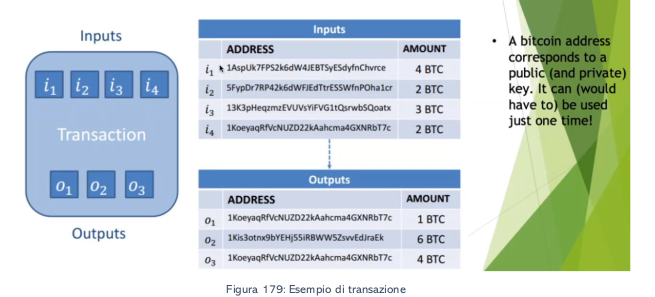
\includegraphics[width=14cm, keepaspectratio]{Bistarelli/img/bitcoin/bit3.png}
\end{figure}

Serie di indirizzi di input (chiavi private) che utilizzo per sbloccare n bitcoin ricevuti in un’unica transazione.
Nell’esempio sopra gli 11 bitcoin in input vengono sbloccati da una determinata chiave privata associata ad una
chiave pubblica e vengono poi inviati agli indirizzi pubblici riportati in output. Ad ogni transazione i bitcoin in input vengono distrutti e vengono creati quelli in output, in questo modo non ci saranno corrispondenze 1 a 1 e i nuovi
non saranno in alcun modo collegati ai vecchi.

\begin{figure}[H]
	\centering
    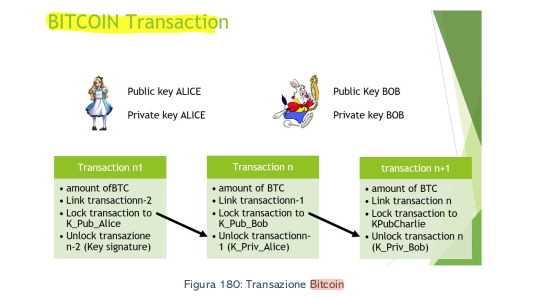
\includegraphics[width=14cm, keepaspectratio]{Bistarelli/img/bitcoin/bit4.png}
\end{figure}

Per scambiare dei bitcoin ogni utente deve creare una coppia di chiavi crittografiche (pubblica e privata) e ad esempio: alice che vuole inviare bitcoin a Bob deve formare una cosidetta transazione bitcoin, nella quale inserire
queste 4 informazioni:

\begin{enumerate}
    \item il numero di bitcoin da inviare
    
    \item indicare al sistema da dove prenderà questi bitcoin inserendo un link ad una transazione che a sua volta ha ricevuto in passato
    
    Poi abbiamo due condizioni crittografiche:
    
    \item lock transaction a favore della chiave pubblica di bob con la quale viene bloccata crittograficamente la transazione a favore della chiave pubblica di Bob indicando di fatto al sistema chi è il nuovo proprietario
    
    \item unlock transaction kprivalice con la quale si da prova al sistema che alice conosce la soluzione alla condizione di lock impostata a suo favore, da qualcun altro, nella transazione $n-1$.
\end{enumerate}
Bob ora ha la transazione N bloccata crittograficamente a suo favore con la possibilità in futuro di formare la
transazione n+1 con la quale cederà i bitcoin a favore di un terzo soggetto. Questo è il modo con cui si scambiano
le proprietà di bitcoin nel sistema. Rimane però in sospeso il fatto che non avendo più a disposizione una parte
centralizzata come una banca chi verifica che le transazioni sono ben formate per poi salvarle nell’archivio
finanziario chiamato blockchain??

\singlespacing

Tutte le transazioni non vengono inviate ai miner ma alla rete in un pool generale, poi saranno i miner a
decidere quale transazione mettere in un blocco.

\singlespacing

Secondo quali regole i miner scelgono queste transazioni?
La regola generale dice che si devono inserire nei blocchi prima le transazioni ad importo maggiore e prima le
transazioni più vecchie. Ad oggi però le regole sono un po' cambiate vista la mole di transazioni in attesa, infatti
se qualcuno vuole può incentivare il miner a prelevare prima la propria transazione. Per incentivare il miner a
prelevarla bisognerà lasciare al miner una piccola commissione (o tassa), per esempio 0,5 bitcoin sugli 11 totali
dell’esempio fatto in precedenza. Nel protocollo è stabilito che quando i miner inseriscono nuove monete ricevono
un compenso, questo compenso è variabile e col tempo verrà decrementato fino ad arrivare a 0 in base al rapporto
compenso-numero di blocchi nuovi inseriti, tutto ciò avviene affinchè i miner si concentrino principalmente
sulle transazioni (dove riceveranno le commissioni degli utenti) e non sull’inserimento di nuove
monete/blocchi. Se così non fosse non sarebbero incentivati e l’ecosistema bitcoin crollerebbe.

\begin{figure}[H]
	\centering
    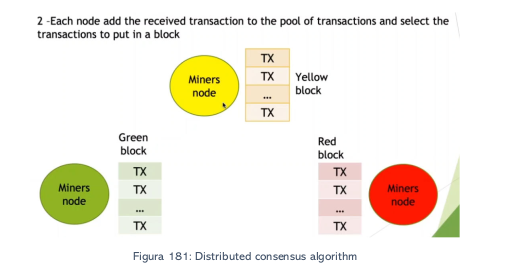
\includegraphics[width=14cm, keepaspectratio]{Bistarelli/img/bitcoin/bit5.png}
\end{figure}

I miner prendono quindi le transazioni dal pool e formano un blocco da inserire nella blockchain. Affinchè tutto
questo avvenga in modo sincrono tra i nodi ( in maniera tale che a tutti risultino le stesse transazioni prelevate e
inserite) c’è bisogno che questi nodi si parlino per capire quali transazioni ogni nodo può prelevare dal pool e
inserire nella blockchain. Il protocolli di consenso regolano questo tipo di operazioni, i più utilizzati nell’ambito
delle criptovalute sono il proof of work (PoW, bitcoin) e il proof of stack (PoS, ethereum a breve).

\begin{enumerate}
    \item Nel proof of work la ricompensa non viene data a tutti i nodi ma al primo che riesce a risolvere un problema crittografico, questo si aggiudicherà il diritto di scegliere quale transazione inserire nel blocco. Per risolvere il problema il miner dovrà trovare una stringa che aggiunta alle transazioni del blocco dia come risultato $00000xxxxxxxxxxx$ una volta hashata. L’unico modo per ottenere la stringa è facendo dei tentativi per indovinarla. Una volta verificata la correttezza della stringa dagli altri nodi l’operazione sarà approvata. La difficoltà per i miner varia in base al numero di 0 iniziali contenuti nella stringa finale, questi 0 possono essere aumentati o diminuiti in base al tempo di risoluzione medio impiegato dai miner (che dovrebbe sempre aggirarsi intorno ai 10 minuti).
\end{enumerate}

\begin{figure}[H]
	\centering
    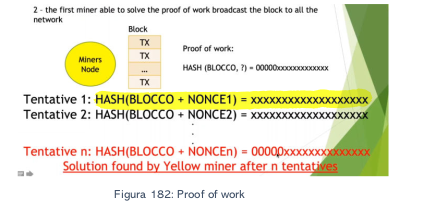
\includegraphics[width=14cm, keepaspectratio]{Bistarelli/img/bitcoin/bit6.png}
\end{figure}

Tra tutte le transazioni inserite il miner aggiunge anche una propria transazione, che viene detta coinbase. A
differenze delle normali transazioni contiene solo l’output, ovvero l'indirizzo Bitcoin del minatore che ha eseguito
con successo il mining del nuovo blocco (e non input e output), questi tipi di transazioni fanno parte del sistema
per mettere in circolazione nuove monete che non sono mai state spese. È grazie a questi tipi di transazioni che
l'ecosistema Bitcoin ha iniziato ad avere criptovalute per effettuare pagamenti e scambi di valore.

\singlespacing

Le transazioni Coinbase sono anche note come generazione di transazioni. Queste sono una parte fondamentale
della generazione delle monete Bitcoin, poiché sono quelle che danno origine a queste nuove monete. Cioè, ogni
transazione coinbase è responsabile della trasmissione delle monete vergini al minatore che ha risolto il blocco.
In questo modo, il valore base totale di a transazione coinbase, contiene solo ed esclusivamente nuove monete
che non sono mai state nel file blockchain

\subsection{Coinbase}
\begin{center}
    \textbf{Caratteristiche coinbase}
\end{center}
Quando un nuovo blocco viene generato sulla blockchain, ha un elenco di transazioni verificate al suo interno.
Ciascuna di queste transazioni è stata generata dagli utenti di criptovaluta di detta blockchain. Ma nonostante, la
prima di queste transazioni corrisponde alla transazione coinbase. Il valore di base di questa transazione è
equivalente a quello della ricompensa attualmente attiva per il mining di quel blocco.
Ciò significa che il valore di questa transazione è legato alla ricompensa del blocco corrente e risente del
dimezzamento attivo in quel momento per quella criptovaluta.

\begin{figure}[H]
	\centering
    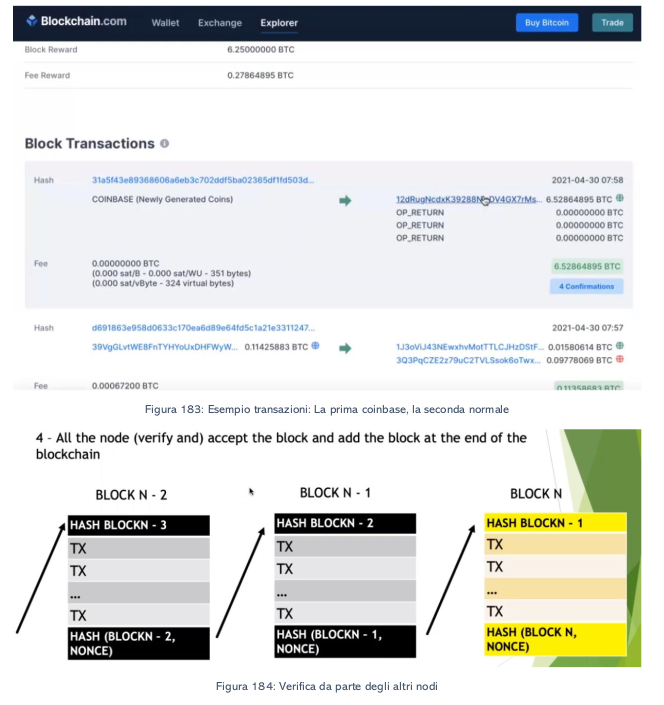
\includegraphics[width=14cm, keepaspectratio]{Bistarelli/img/bitcoin/bit7.png}
\end{figure}

\begin{figure}[H]
	\centering
    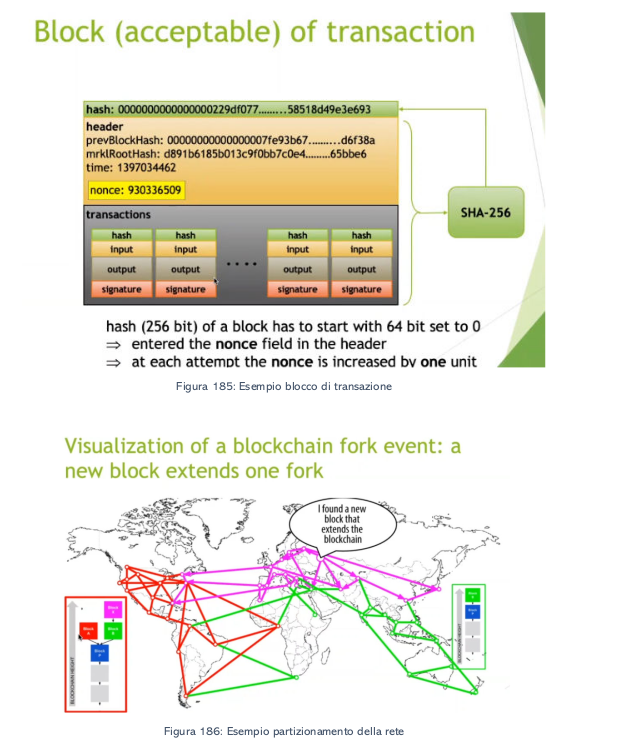
\includegraphics[width=14cm, keepaspectratio]{Bistarelli/img/bitcoin/bit8.png}
\end{figure}

Se un’identica transazione venisse inserita e gestita prima da una parte della rete (nell’esempio rossa o verde) si
verrebbero a creare due partizioni della rete non sincronizzate con problemi di integrità e consistenza. Questi
problemi si risolvono con una semplice regola: la blockchain a cui fare riferimento è sempre quella più lunga,
nel caso dell’esempio il blocco rosso viene scartato e si prosegue sull’altra via, quella viola (blocco x). Queste
situazioni durano in media 10 minuti, ovvero il tempo di inserimento/aggiornamento tipico della catena
blockchain. Potrebbe in rari casi durare al massimo un’ora, perciò un blocco viene considerato inserito al 100%
(quindi non potrà più essere cancellato) solo quando si trova al livello 6-7 della catena (dopo 6-7 aggiornamenti
da 10 minuti).

\begin{figure}[H]
	\centering
    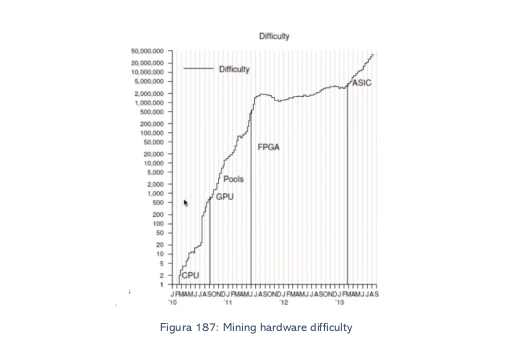
\includegraphics[width=14cm, keepaspectratio]{Bistarelli/img/bitcoin/bit9.png}
\end{figure}

Negli anni la difficoltà di risolvere i problemi e minare è sempre aumentata, questo perché la competitività e i
requisiti hardware dei miner sono aumentati (e continueranno a farlo) con l’aumentare dei prezzi dei bitcoin. I
miner hanno la possibilità di “unire le forze” con altri miner (Pools), in modo tale da compensare o aumentare la
potenza di calcolo, in tal caso le ricompense saranno distribuite in base al contributo dato.
Gli ASIC sono architetture create apposta per calcolare gli hash.
La tecnologia FPGA (Field Programmable Gate Array) è stata praticamente sostituita dall’ASIC.

\begin{figure}[H]
	\centering
    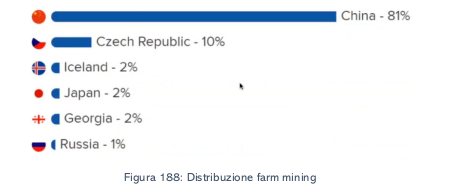
\includegraphics[width=14cm, keepaspectratio]{Bistarelli/img/bitcoin/bit10.png}
\end{figure}

La distribuzione della farm è fortemente condizionata dal costo della corrente, per questo motivo l’81% di queste
farm/miner è situata in Cina. La distribuzione delle potenze di calcolo o dell’ambiente distribuito va tenuta sempre
sotto controllo a livello globale, in modo tale da distribuire equamente la potenza e il potere ai vari nodi della rete
(che appunto deve mantenere l’equilibrio di una rete distribuita).

\subsection{Dettagli su come si sbloccano le transazioni}

\begin{figure}[H]
	\centering
    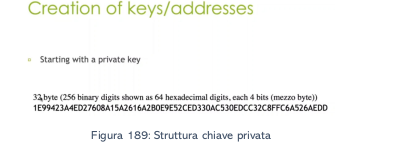
\includegraphics[width=14cm, keepaspectratio]{Bistarelli/img/bitcoin/bit11.png}
\end{figure}

Una chiave privata è composta da 32 byte. A partire dalla chiave privata tramite curve ellittiche si calcola la chiave
pubblica, dalla chiava pubblica con la funzione di hash si utilizza un idirizzo bitcoin.

\begin{figure}[H]
	\centering
    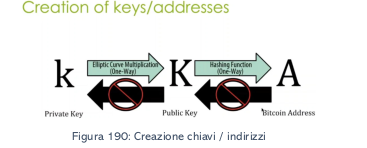
\includegraphics[width=14cm, keepaspectratio]{Bistarelli/img/bitcoin/bit12.png}
\end{figure}

A partire dalla chiave privata per ottenere la chiave pubblica si moltiplica la chiave private un tot di volte fino ad
ottenere la chiave pubblica.

\begin{figure}[H]
	\centering
    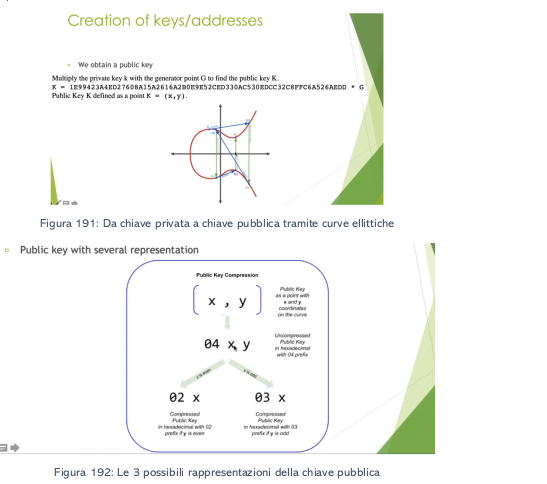
\includegraphics[width=14cm, keepaspectratio]{Bistarelli/img/bitcoin/bit13.png}
\end{figure}

Da questa chiave pubblica con una funzione di hashing ottengo l’indirizzo bitcoin da inserirre nelle transazioni.

\begin{figure}[H]
	\centering
    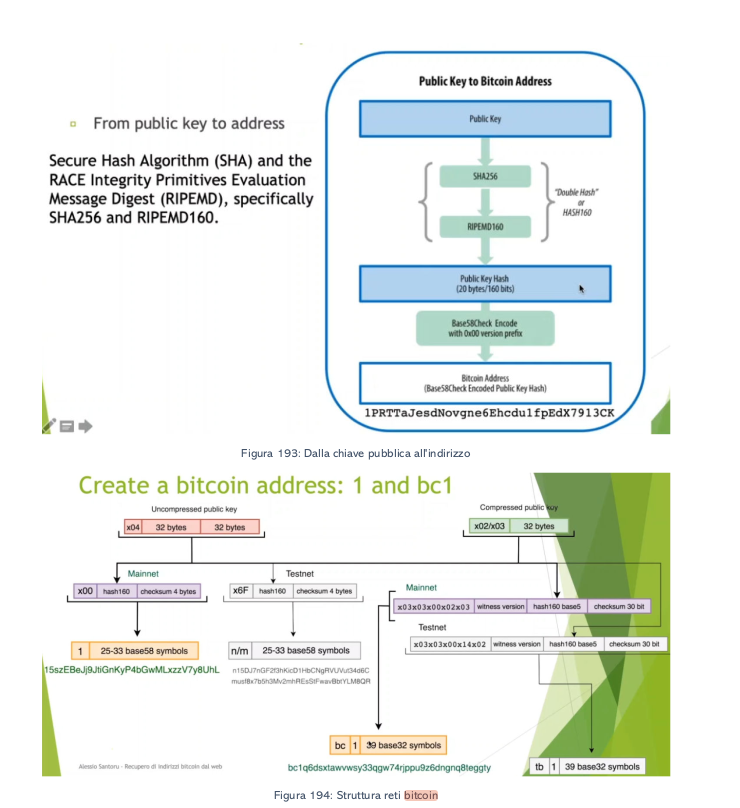
\includegraphics[width=14cm, keepaspectratio]{Bistarelli/img/bitcoin/bit14.png}
\end{figure}

La struttura delle reti bitcoin comprende anche una “Testnet” dove effettuare delle prove locali che non verranno
applicate alla rete.
Negli anni è cambiata la maniera di calcolare i bitcoin, quella più utilizzata in questo momento è “bc | 1 | 39
base32 symbols”.

\begin{figure}[H]
	\centering
    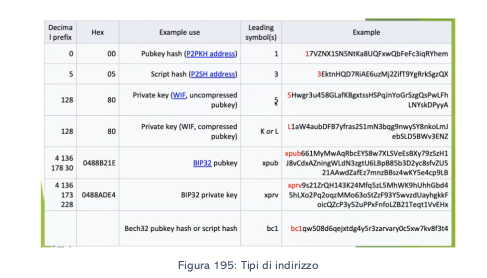
\includegraphics[width=14cm, keepaspectratio]{Bistarelli/img/bitcoin/bit15.png}
\end{figure}

Una transazione può essere sbloccata in 5 modi diversi:

\begin{enumerate}
    \item Ti pago se tu mi dimostri di avere una determinata chiave privata corrispondente ad una chiave pubblica
    
    \item Ti pago se dimostri di avere questa chiave pubblica
    
    \item Transazioni che non possono essere mai sbloccate, i bitcoin vengono persi
    
    \item  Vengono spesso utilizzate per certi tipi di contratti in bitcoin, posso richiedere che la transazione venga sbloccata solo se vengono (per esempio) fornite 2-3 chiavi su 5 che sto richiedendo
    
    \item Io faccio un script hash e ti pago se tu dimostri di conoscere qual è la stringa il cui hash ti da quello che dico io
\end{enumerate}


\begin{figure}[H]
	\centering
    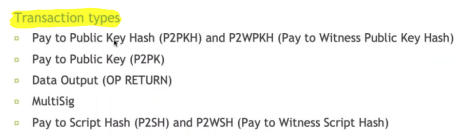
\includegraphics[width=14cm, keepaspectratio]{Bistarelli/img/bitcoin/bit16.png}
\end{figure}

\subsection{Pay to Public Key Hash (P2PKH)}
Lo sblocco di una transazione inviata ad una chiave pubblica non si fa mostrando e rivelando la chiave privata ma
si fa firmando questa transazione con la chiave privata, mostrando poi questa firma al sistema. Infine il sistema
verifica se la firma è corretta applicando la chiave pubblica a questa firma per vedere se ottiene questa transazione.

\begin{figure}[H]
	\centering
    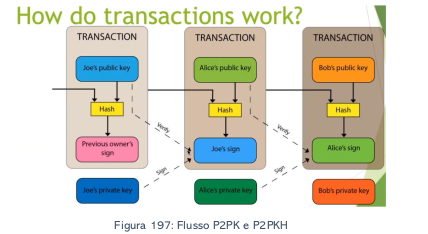
\includegraphics[width=14cm, keepaspectratio]{Bistarelli/img/bitcoin/bit17.png}
\end{figure}

\begin{figure}[H]
	\centering
    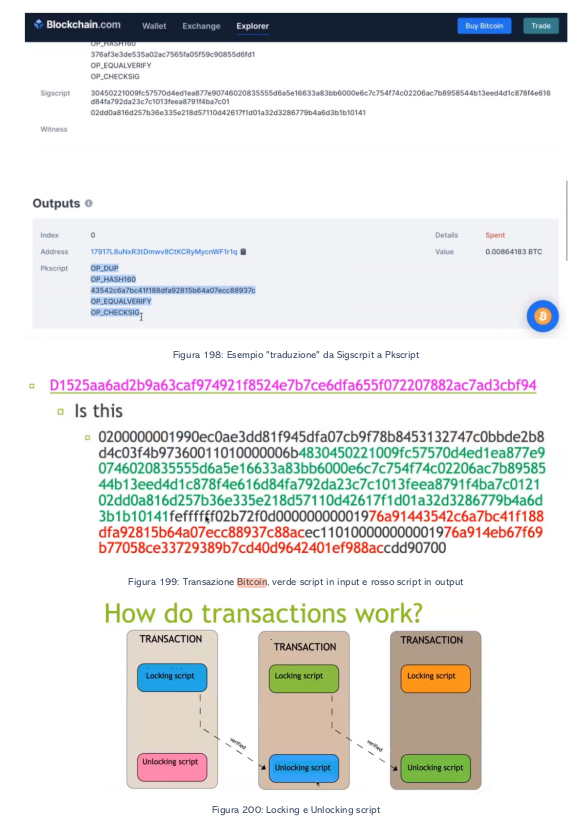
\includegraphics[width=14cm, keepaspectratio]{Bistarelli/img/bitcoin/bit18.png}
\end{figure}

Come fa una transazione con un determinato input a sbloccare un determinato output? Si deve intrepetare l’input
a coppie esadecimali come delle istruzioni assembler.

\begin{figure}[H]
	\centering
    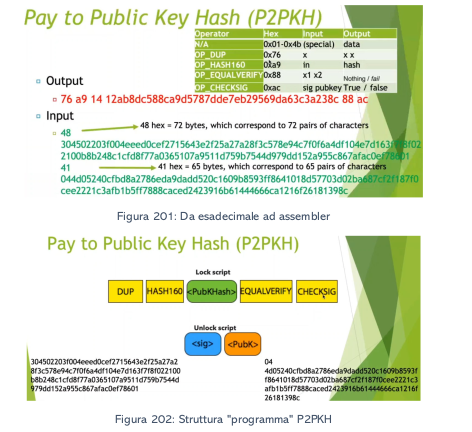
\includegraphics[width=14cm, keepaspectratio]{Bistarelli/img/bitcoin/bit19.png}
\end{figure}

Se concateniamo l’unlock script al lock script (output e input) otteniamo un programma con il flusso di istruzioni
riportato nell’immagine precedente. Il linguaggio di scripting utilizzato è chiamato bitcoin script.

\singlespacing

E' non touring complete perché non ha i cicli, utile come meccanismo di difesa (ddos, brute force). Ethereum
li ha ma ha un meccanismo per limitarli e non renderli infiniti.

\begin{figure}[H]
	\centering
    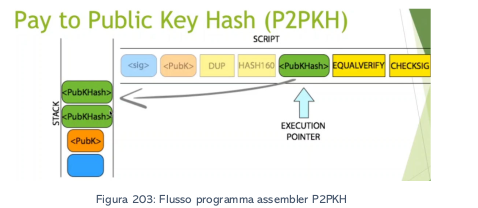
\includegraphics[width=14cm, keepaspectratio]{Bistarelli/img/bitcoin/bit20.png}
\end{figure}

\begin{enumerate}
    \item Metto nello stack i 48 hex (72 bytes dell’input)
    
    \item Inserisco e duplico la chiave pubblica
    
    \item Effettuo l’hash sulla chiave pubblica
    
    \item Metto sullo stack la chiave pubblica
    
    \item Eseguo equal verify per vedere se la chiave pubblica è uguale alla chiave pubblica duplicata
    
    \item Eseguo equal verify per vedere se la chiave pubblica corrisponde alla signature
    
    \item Se è tutto true la transazione verrà sbloccata e completata
\end{enumerate}

chainquery.com -> dato un id di una transazione restituisce la transazione

\begin{figure}[H]
	\centering
    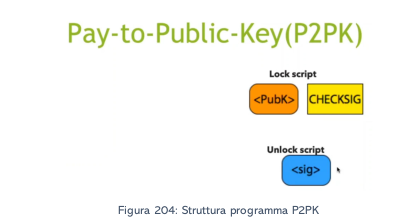
\includegraphics[width=14cm, keepaspectratio]{Bistarelli/img/bitcoin/bit21.png}
\end{figure}

La P2PKH è la transazione più utilizzata, è preferita alla P2PK perché occupa meno spazio nella transazione. Lo
spazio nel blocco è fisso, quindi utilizzando una P2PKH e non una P2PK un blocco potrebbe contenere un numero
maggiore di transazioni.

\subsection{M-of-N Multi-signature (multisig)}
Il pagamento avviene a condizione di fornire n signature su un tot di m chiavi pubbliche fornite.

\begin{figure}[H]
	\centering
    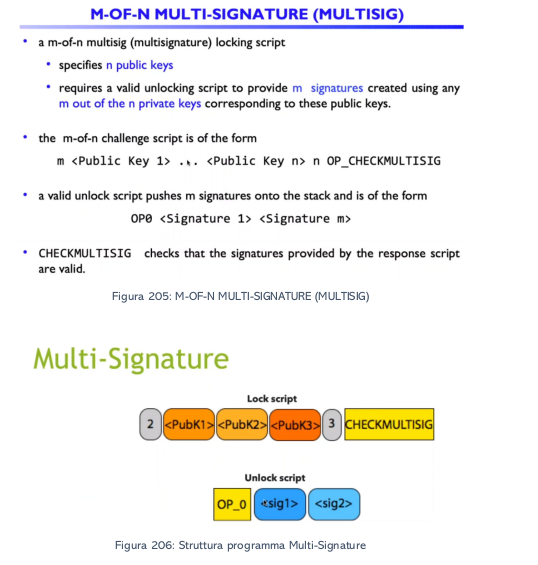
\includegraphics[width=14cm, keepaspectratio]{Bistarelli/img/bitcoin/bit22.png}
\end{figure}

\begin{figure}[H]
	\centering
    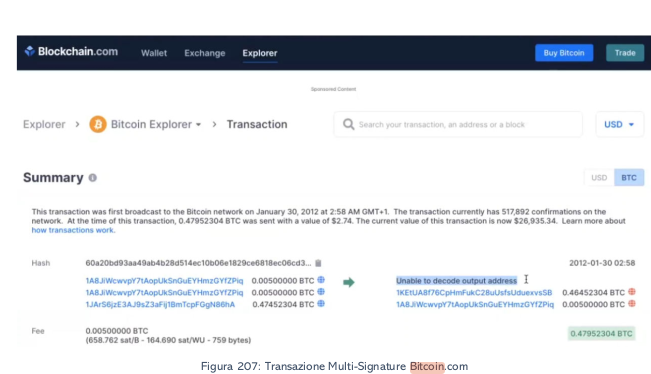
\includegraphics[width=14cm, keepaspectratio]{Bistarelli/img/bitcoin/bit23.png}
\end{figure}

La parte di transazione evidenziata è multi-signature perché non si riesce a risalire agli indirizzi di output. Si verrà
a conoscenza dell’indirizzo solo quando verrà sbloccato, ovvero quando 2 indirizzi su 3 verranno sbloccati e il
denaro verrà inviato a quei 2 indirizzi, nel momento iniziale in cui inserisce la transazione non si è a conoscenza
degli indirizzi di output.
Uso delle multi-signature:
\begin{itemize}
    \item 1-of-n: qualunque utente (che fa parte degli n utenti) può spendere il denaro ma è importante tenere traccia di chi l’ha fatto
    
    \item 2-of-2: solo se entrambe le parti coinvolto è d’accordo con la spessa la transazione viene sbloccata
    
    \item 2-of-3: contratti di vendita garantiti da una terza parte fidata, quindi 3 chiavi pubbliche coinvolte. Anche detti escrow contract (in italiano deposito di garanzia). 
    
    Es. Se A deve inviare soldi a B, C tiene i soldi di A e non li da a B finchè B non da ad A quello che gli spetta, in questo caso scambio di soldi e signature.
\end{itemize}

\begin{figure}[H]
	\centering
    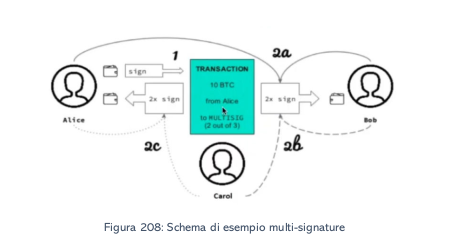
\includegraphics[width=14cm, keepaspectratio]{Bistarelli/img/bitcoin/bit24.png}
\end{figure}
Esistono anche le transazioni con il lock time, dove A paga B dopo solo dopo un tempo T. 

\singlespacing

La multi-signature permette di fare una prima forma di smart contact, però occupando tanti “posti” (chiavi
numerose) non viene preferita, un’alternativa è fare l’hash dello script in modo tale che occupi meno spazio (Pay
to Script Hash, P2SH).

\begin{figure}[H]
	\centering
    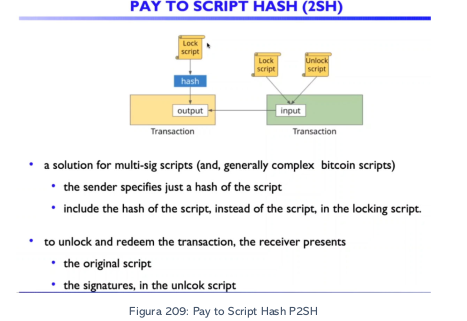
\includegraphics[width=14cm, keepaspectratio]{Bistarelli/img/bitcoin/bit25.png}
\end{figure}

Nella transazione di output che blocca inserisco uno script di Lock e poi faccio l’hash, dalla parte dell’input invece
viene fatto il lock script per verificare che le stringhe hash generate dai due Lock Script corrispondano e poi viene
eseguito lo script di unlock se tutto da TRUE.

\begin{figure}[H]
	\centering
    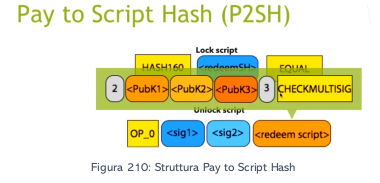
\includegraphics[width=14cm, keepaspectratio]{Bistarelli/img/bitcoin/bit26.png}
\end{figure}

Di solito nello script di redeem (riscatto) c’è una P2PK .

\subsection{Data Output (OP Return)}

Vengono utilizzate normalmente per scrivere in blockchain ed avere garanzie di notarizzazione.

\singlespacing

Ogni elemento scritto di blockchain ha una data e orario, quindi hashato sarà univoco

\singlespacing

Come funziona la OP Return? Si mette un indirizzo a caso di 20 byte che è un pagamento fake che non può
essere mai speso e si inserisce una parte di dato che corrisponde per esempio all’hash del programma/transazione
di cui voglio dimostrare l’esistenza. OP\_RETURN <data> dove “data” sono i dati che io voglio dimostrare.

\begin{figure}[H]
	\centering
    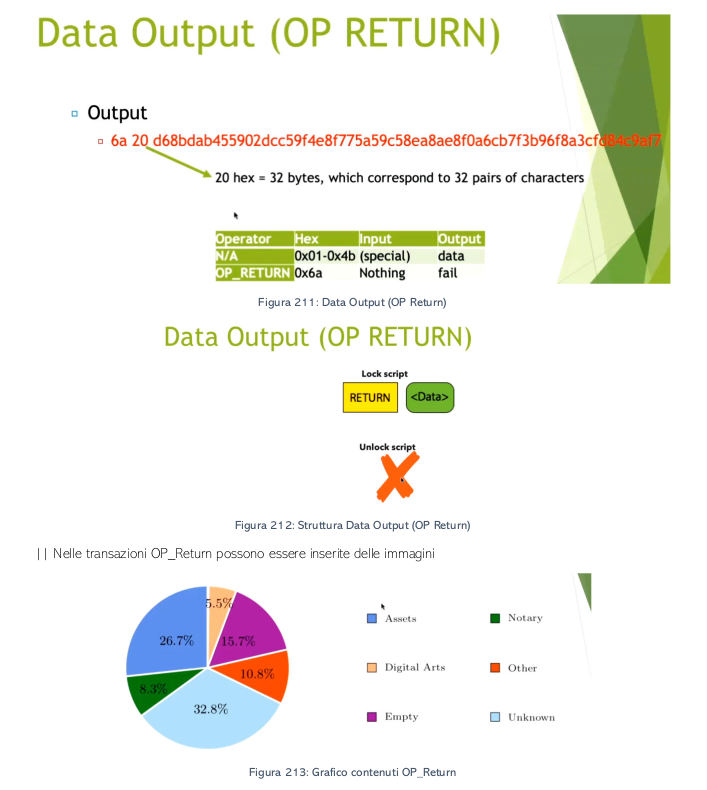
\includegraphics[width=14cm, keepaspectratio]{Bistarelli/img/bitcoin/bit27.png}
\end{figure}

\begin{figure}[H]
	\centering
    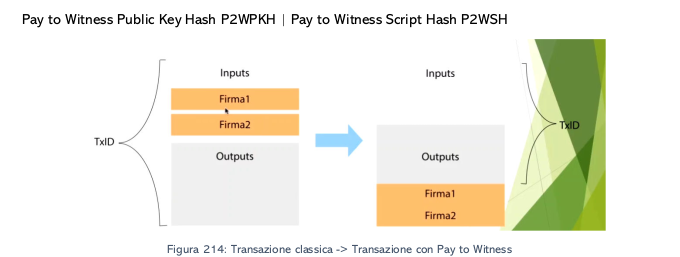
\includegraphics[width=14cm, keepaspectratio]{Bistarelli/img/bitcoin/bit28.png}
\end{figure}

Se le firme di una transazione vengono scritte in maniera diversa (ci sono più modi per scriverle) l’hash generato
sarà ovviamente diverso anche se la transazione è la stessa, questa problematica viene chiamata transaction
malleability.

\singlespacing

Per evitare questo problema si è deciso di spostare le firme fuori dalle transazioni da firmare/hashare. L’altra
modifica che viene fatta è togliere gli script di input e di output, perché si sa qual è l’operazione da fare per
controllare la firma,
Quindi perché viene adottata? Risparmio di spazio e difesa da attacchi/problematiche di transaction malleability.

\begin{figure}[H]
	\centering
    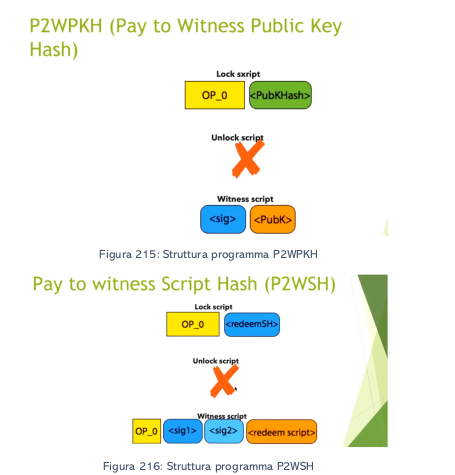
\includegraphics[width=14cm, keepaspectratio]{Bistarelli/img/bitcoin/bit29.png}
\end{figure}

I 5 tipo di transazione appena descritte vengono chiamate “transazioni standard”. Dal momento che uno script
bitcoin potrebbe contenere qualsiasi cosa, i miner posso anche decidere di minare “non standard”.

\subsection{Contenuti tipici transazioni non strandard}

\begin{figure}[H]
	\centering
    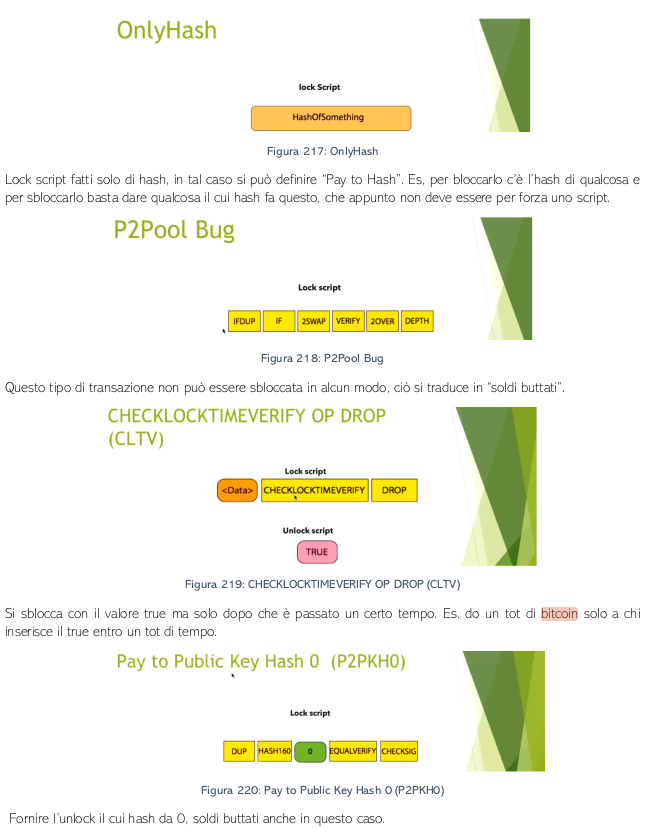
\includegraphics[width=14cm, keepaspectratio]{Bistarelli/img/bitcoin/bit30.png}
\end{figure}

\begin{figure}[H]
	\centering
    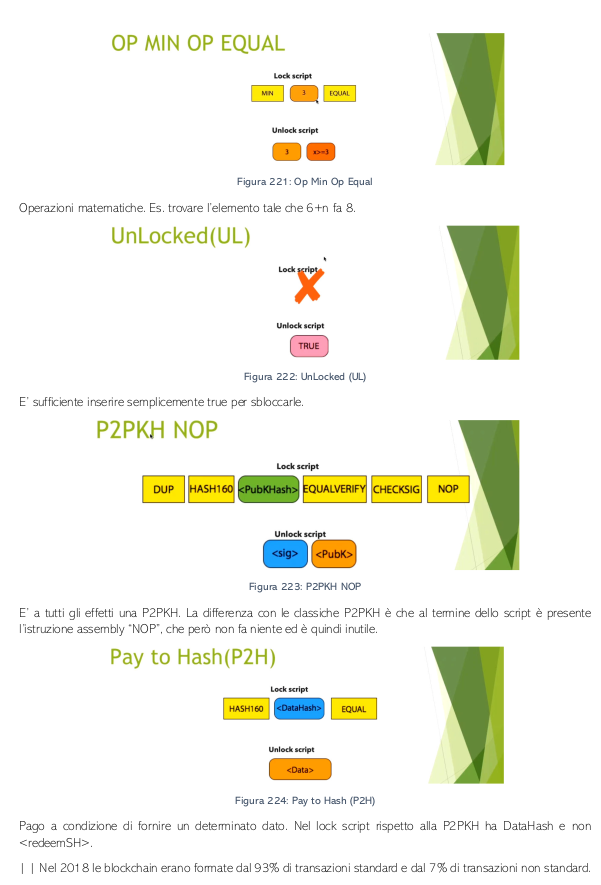
\includegraphics[width=14cm, keepaspectratio]{Bistarelli/img/bitcoin/bit31.png}
\end{figure}

\begin{figure}[H]
	\centering
    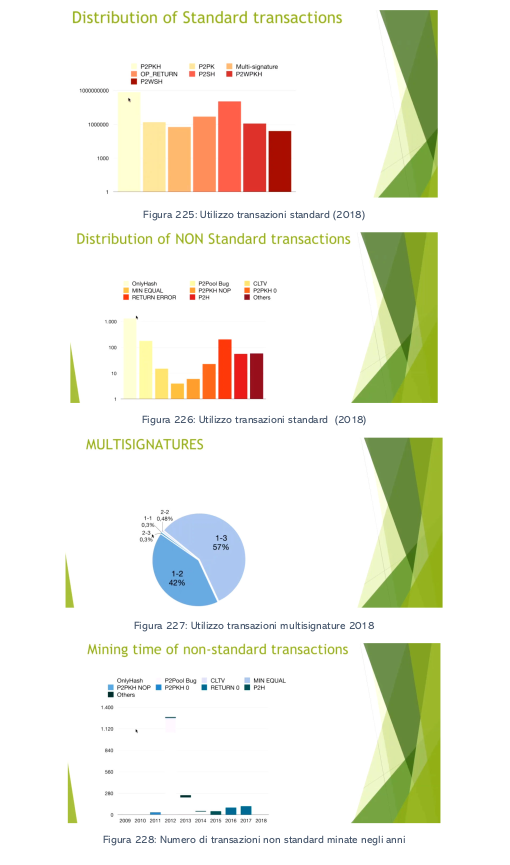
\includegraphics[width=14cm, keepaspectratio]{Bistarelli/img/bitcoin/bit32.png}
\end{figure}

\begin{figure}[H]
	\centering
    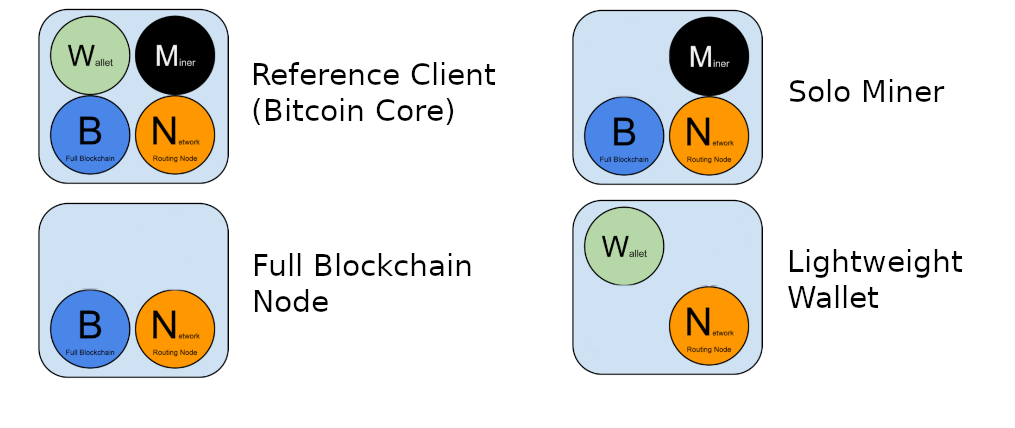
\includegraphics[width=14cm, keepaspectratio]{Bistarelli/img/bitcoin/bit33.png}
\end{figure}

\subsection{Sicurezza della blockchain}
Ransom attack: sfrutta il fatto che bitcoin è pseudoanonimo e non completamente anonimo. (non si sa a chi è
associata una chiave pubblica) (Attacco + riscatto)

\singlespacing

51\% attack: sfrutta problema dovuto al protocollo di consenso (es. proof of work PoW)

\begin{figure}[H]
	\centering
    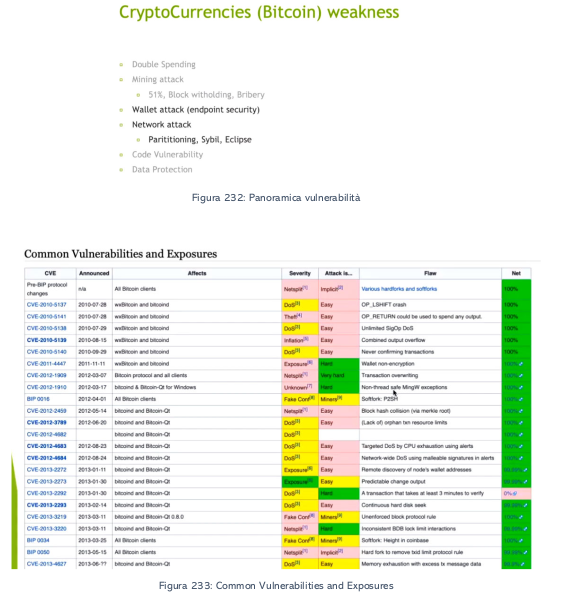
\includegraphics[width=14cm, keepaspectratio]{Bistarelli/img/bitcoin/bit34.png}
\end{figure}

\begin{figure}[H]
	\centering
    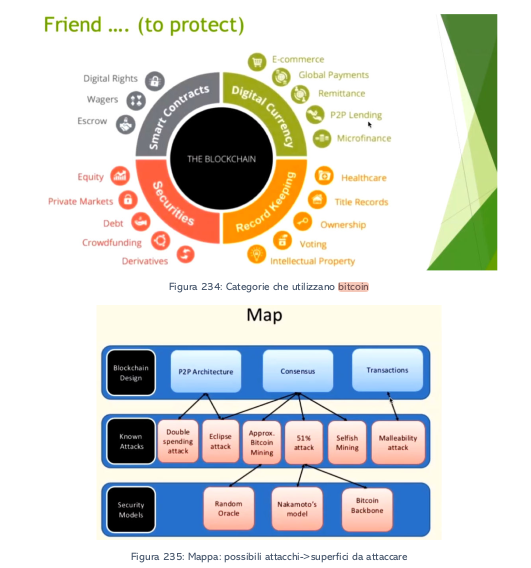
\includegraphics[width=14cm, keepaspectratio]{Bistarelli/img/bitcoin/bit35.png}
\end{figure}

\subsection{Double Spending}
A acquista un bene tramite internet con pagamento bitcoin, A riceve il bene da B e poi invia/divulga tanti blocchi
minati (dopo che i blocchi sono stati minati vengono messi da parte aspettando di essere inviati tutti in una volta)
in modo tale che la catena diventi tanto lunga da sovrascrivere le operazioni precedenti e annullare la transazione.
Ad oggi è molto difficile realizzare questo tipo di attacchi vista la dimensione della rete e le elevate potenze di
calcolo richieste. Questo è attacco è stato fatto da “Finney”.

\singlespacing

La soluzione più comune prevede che B consegni la merce acquistata da A soltanto dopo che la transazione è
stata scritta in blockchain dai miner, quindi non basta che la transazione venga inviata da A al pool (il passaggio
successivo al pool è appunto l’aggiunta in blockchain da parte dei miner). Per evitare anche il caso estremo del
partizionamento della rete si potrebbe anche aspettare che la transazione raggiunga prima il sesto-settimo blocco,
quindi 60-70 minuti in modo tale che non possa essere sovrascritta dal percorso più lungo.

\begin{figure}[H]
	\centering
    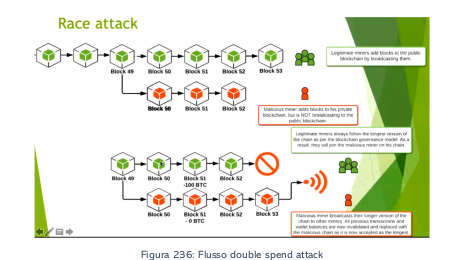
\includegraphics[width=14cm, keepaspectratio]{Bistarelli/img/bitcoin/bit36.png}
\end{figure}

A porta avanti due flussi di transazioni in parallelo minando le transazioni a due livelli (verde e rosso), appena A
riceve la merce da B (flusso verde) effettua il broadcast delle transazioni minate di nascosto sul flusso rosso.
Appena il broadcast viene diffuso il flusso verde viene sovrascritto in quanto più corto e non divulgato, quindi i
soldi non vengono realmente spesi. E’ rarissimo se non impossibile che nel bitcoin (a differenza di monete
emergenti dove le blockchain sono ancora di piccole dimensioni) questo attacco vada a buon fine, nessuno
disporrebbe della potenza di calcolo richiesta per attaccare una blockchain di tali dimensioni.

\begin{figure}[H]
	\centering
    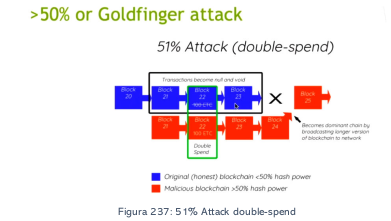
\includegraphics[width=14cm, keepaspectratio]{Bistarelli/img/bitcoin/bit37.png}
\end{figure}

Se ho il 51\% di potenza di calcolo, oltre al double spend posso fare molti altri tipi di attacco, posso praticamente
riscrivere le regole della blockchain. Es. posso cambiare dimensioni e regole delle transazioni. Es. posso effettuare
short selling, ovvero pilotare il prezzo del bitcoin a mio piacimento. Es. posso distruggere completamente la
moneta.

\singlespacing

Il governo cinese potrebbe decidere di impossessarsi dell’80\% della rete visto che la maggior parte delle farm è
situata in Cina, così facendo avrebbe il controllo assoluto sul bitcoin.

\singlespacing

Per evitare il 51\% attack i detentori dei pool hanno stretto un patto fissando dei limiti alla distribuzione delle
potenze di calcolo. || Nel 2018 la potenza computazionale della rete bitcoin era 7648 volte più grande del
computer più potente del mondo.

\begin{figure}[H]
	\centering
    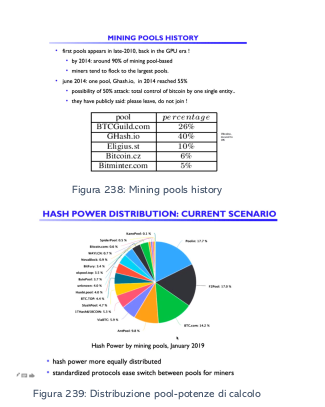
\includegraphics[width=14cm, keepaspectratio]{Bistarelli/img/bitcoin/bit38.png}
\end{figure}

Esistono siti che vendono anche le potenze di calcolo. Per un utente quasi impossibile acquistarne una quantità
per la moneta bitcoin.

\subsection{Wallet Attack}

Sono attacchi che colpiscono il software che gestisce le chiavi pubbliche e private, il wallet. Avere il wallet non è
una cosa obbligatoria per gestire le blockchain, però vista la mole delle chiavi da gestire è praticamente
indispensabile. L’attacco può avvenire sulla macchina dell’utente che utilizza il wallet oppure sull’exchange server
dove l’utente è registrato.

\singlespacing

Come si fa a gestire bene un wallet?
Quando avviene uno scambio di denaro in criptovaluta e si deve fare una transazione bisogna mandarla a un
nostro indirizzo pubblico gestito da noi sui nostro wallet. Il wallet potrebbe essere un software sul cellulare o su
un computer, ma la cosa migliore è avere dei wallet esterni/token crittografici esterni da sbloccare con pin (è
come quando accediamo ad una smart card), così se uno ruba il dispositivo e riesce a sbloccarlo non può
comunque accedere ai dati contenuti dentro. Con la tecnica della split key la chiave viene memorizzata su device
diversi, quindi l’attacco andrebbe portato a termine su più device e non soltanto su uno.

\begin{figure}[H]
	\centering
    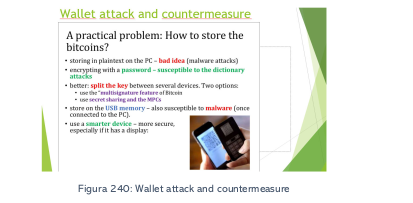
\includegraphics[width=14cm, keepaspectratio]{Bistarelli/img/bitcoin/bit39.png}
\end{figure}

\subsection{Transaction Malleabilit}

Sfrutta il fatto che una parte della transazione è firmata con la chiave privata del possessore dei fondi. Ogni
transazione è unicamente identificata da un hash, questo hash non è calcolato solo sui dati finanziari ma anche
sulla firma (che può essere scritta in modi diversi). Soluzione possibile: witness, transazioni SegWit (Segregated
Witness).

\begin{figure}[H]
	\centering
    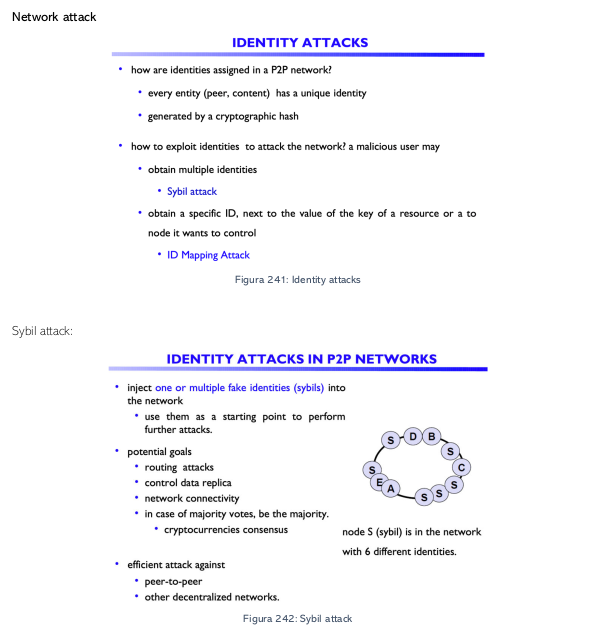
\includegraphics[width=14cm, keepaspectratio]{Bistarelli/img/bitcoin/bit40.png}
\end{figure}

\begin{figure}[H]
	\centering
    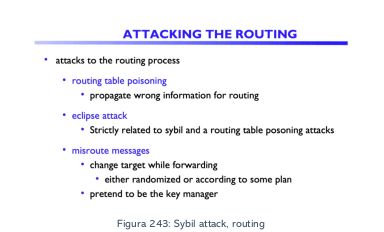
\includegraphics[width=14cm, keepaspectratio]{Bistarelli/img/bitcoin/bit41.png}
\end{figure}

Routing: creando ed impersonando diversi nodi della rete l’attacante può collegarli ad un determinato nodo in
modo tale che venga isolato dagli altri.

\singlespacing

Eclipse: nasconde il resto della rete al nodo stesso, cosi tutti i nodi che sono collegati a lui (quelli che ha creato
l’attaccanto) possono gestire a loro piacimento il routing (routing table poisoning).

\subsection{Code vulnerability}

Vulnerabilità del codice e/o del software.

\begin{figure}[H]
	\centering
    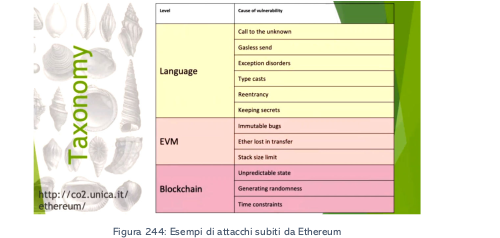
\includegraphics[width=14cm, keepaspectratio]{Bistarelli/img/bitcoin/bit42.png}
\end{figure}

Gli smart contracts sono i principali destinatari degli attacchi software.
I contratti una volta messi in blockchain sono immutabili, trasparenti (tutti possono guardare il codice), vengono
eseguiti in maniera autonoma (quando per esempio scattano degli eventi) e si possono controllare sempre visto
che rimagono in blockchain. Con gli smart contract si può eseguire della computazione o trasferire del denaro, in
ethereum hanno anche un indirizzo pubblico dedicato come per gli utenti.

\begin{figure}[H]
	\centering
    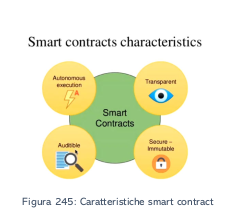
\includegraphics[width=14cm, keepaspectratio]{Bistarelli/img/bitcoin/bit43.png}
\end{figure}

Caso DAO attack (Decentralized Autonomous Organization)

\singlespacing

Era uno smart contract che permetteva di effettuare transazioni senza utilizzo di moneta, uno dei metodi era
bacato e poteva essere chiamato più volte senza fare un controllo. Un utente sfruttò questo metodo per indirizzare
tanti smart contract a se stesso, i contratti però non potevano essere cambiati in quanto immutabili. L’unica
soluzione era fare una sorta di roll back di tutti i blocchi inseriti prima e ripartire, non tutti però erano ovviamente
d’accordo. Alla fine la rete si è divisa in due mondi: Ethereum ed Ethereum Classic, i primi hanno effettuato il
roll back ed hanno corretto il baco, i secondi no.

\begin{figure}[H]
	\centering
    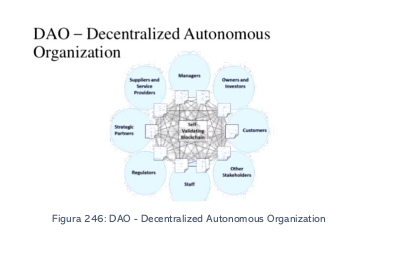
\includegraphics[width=14cm, keepaspectratio]{Bistarelli/img/bitcoin/bit44.png}
\end{figure}

